\documentclass{sig-alternate}
\usepackage{url}

%% Bring items closer together in list environments
% Prevent infinite loops
\let\Itemize =\itemize
\let\Enumerate =\enumerate
\let\Description =\description
% Zero the vertical spacing parameters
\def\Nospacing{\itemsep=0pt\topsep=0pt\partopsep=0pt\parskip=0pt\parsep=0pt}
% Redefine the environments in terms of the original values
\renewenvironment{itemize}{\Itemize\Nospacing}{\endlist}
\renewenvironment{enumerate}{\Enumerate\Nospacing}{\endlist}
\renewenvironment{description}{\Description\Nospacing}{\endlist}

\begin{document}
\conferenceinfo{UWCSE503}{'10 Seattle, WA USA}

\title{JavaGrok: Automatic Inference of Documentation for Under-documented Code}

\numberofauthors{1} 
\author{
\alignauthor
Colin S. Gordon, Reto Conconi, Gilbert Bernstein, Michael Bayne\\
       \affaddr{University of Washington}\\
       \affaddr{Seattle, WA USA}\\
       \email{\{csgordon,conconir,gilbo,mdb\}@cs.washington.edu}
}

\maketitle
\begin{abstract}
Modern software development increasingly involves the use of third party
libraries. Developers now routinely locate and learn the APIs of myriad
libraries in the course of a single software development project. This process
is made more difficult by the fact that many libraries are poorly documented.
The developer often has to read the library source code or resort to trial and
error to determine how to correctly use the library. These methods of learning
about the library are time consuming and error prone.

We present a method to automatically augment library API documentation with invariants
inferred by a variety of static analyses. These include argument nullability,
argument and receiver mutation, argument leaking and capturing, and conditions
that will cause exceptions to be thrown.

We also present a manual comparison of inferred information against an existing
code base considered to have good documentation, and perform a user study to
evaluate the usefulness of the additional documentation for developers.
\end{abstract}

% These categories are from the ACM CCS (Computing Classification System)
% http://portal.acm.org/ccs.cfm
\category{F.3.1}{Specifying and Verifying and Reasoning about
Programs}{Specification techniques}
\category{D.2.7}{Distribution, Maintenance, and Enhancement}{Documentation}
\category{D.2.13}{Software Engineering}{Reusable Software}

% These "terms" are from the ACM's official General Terms classifications.
% http://www.acm.org/about/class/1998
\terms{Documentation, Human Factors, Languages}

\keywords{Documentation Inference, Software Documentation, Static Analysis}

\section{Introduction}

Despite their best intentions, many developers routinely fail to provide adequate or any documentation of the code they write.  Whether because of bad practice, laziness or a sincere belief on the part of programmers that their code will soon be thrown away, much code in regular use and reuse remains undocumented.  New developers join the team, the code gets handed off to another group, or perhaps even posted publicly on the internet.  By various means, this code finds its way into the hands of programmers who---having been assured that this code will save them weeks of effort---now face a thoroughly unenviable task: grok a lump of un(der)documented code and figure out its interface enough to solve their original problem.

Ideally, we would have an army of ingenious, classically trained Shakespearean typing monkeys, ready to provide high-quality documentation for all our programs and libraries at the drop of a hat.  However in reality, we, the unlucky developers often must make do with a single use case or oblique e-mail offering advice---if we are even that lucky.  Sitting at our desks, we curse fate, the code in front of us, and the anonymous (or not so anonymous) programmer responsible for our pain.  We wonder, wouldn't it be nice if we could just push a button and get some useful, if not perfect documentation?

We designed a tool, named JavaGrok, to do just this: take an un(der)documented library and opportunistically infer bare-bones documentation to aid a client programmer.  Our tool takes a collection of java source files intended for use as a library, computes a variety of modular static analyses, and then places select results from these analyses into the javadoc documentation for the provided classes.  These analysis results appear side by side, line by line with any pre-existing documentation.  They warn the library's user about potentially null return values, possible side-effects and unhandled exceptions, to name a few examples.  Armed with this reinforced documentation, our unfortunate programmer is now ready to do battle with their unseemly library.

Certainly, any attempt to provide automatically generated documentation is prone to being useless or even actively unhelpful if done incorrectly.  In order to verify that the provided automatic documentation helps rather than hurts users, we have conducted a user study.  Programmers were asked to accomplish a routine task(?) using an unfamiliar library and lacking extensive or robust documentation.  It turns out we discovered some interesting results.  Go us!

\section{Technical Approach}
To infer information about Java code we use existing inference tools and
combine their output. We have additionally developed a simple framework to aid
in writing our own analyses, should that prove necessary.

To combine the results of disparate analyses we have to convert their results
into a common format at some point in our toolchain.  We will use the JAIF
(Java Annotation Index File) format for that purpose.  Some anaylses generate
results directly in JAIF format, some provide annotated bytecodes which can be
easily extracted into JAIF format, and others provide textual results for which
we will write simple translators into JAIF format.

\begin{figure}
\centering
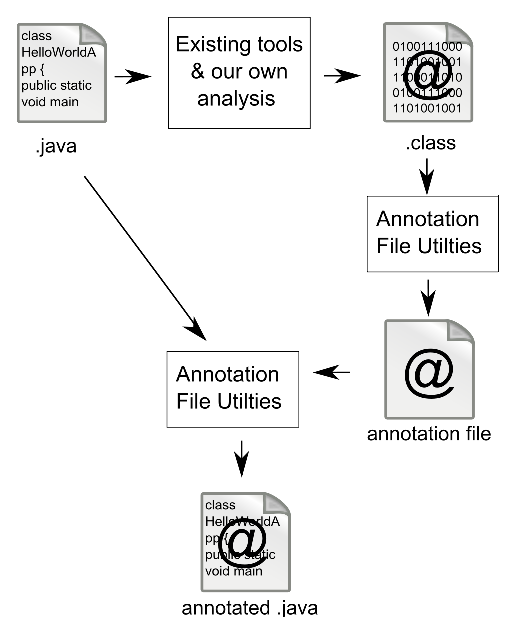
\psfig{file=figures/technicalApproach/technicalApproach.eps, width=3in}
\caption{Toolchain}
\label{fig:toolchain}
\end{figure}

In the following section we describe our simple analysis framework.  In
sections~\ref{sec:Javarifier} through~\ref{sec:Nullability} we describe each of
the existing analyses we will be using in our evaluation and how we will
integrate its results into our toolchain. In the section~\ref{sec:jaif2html} we
explain the final step of our process which is to integrate the various
analysis into the Javadoc generation process.

Figure \ref{fig:toolchain} shows the stages in our toolchain.

\subsection{Analysis Framework}
\label{ss:analysisFramework}

To implement our own analysis tools we use the Annotation Processing Tool (APT)
API~\cite{apt} built into the Java standard compiler.  From within an APT plugin
we can access the compiler's abstract syntax tree and augment the generated
bytecode with annotations representing our analysis results. These annotations
are then extracted into external annotation files.

\subsection{Javarifier}
\label{sec:Javarifier}

Javarifier is a tool to infer reference immutability information built in
conjuction with research done by Quinonez et al.~\cite{Javarifier}. It infers
mutability constraints for object fields, method arguments and receivers. Those
constraints may be \texttt{mutable}, \texttt{readonly}, \texttt{?~readonly},
\texttt{polyread}, and \texttt{this-mutable}. The \texttt{?~readonly}
constraint indicates a method argument with a \texttt{readonly} upper bound and
a \texttt{mutable} lower bound. The \texttt{polyread} constraint provides
polymorphism over mutability for method arguments and receivers
(i.e. indicating that a method is read-only when called through a read-only
reference or mutable when called through a mutable reference). A
\texttt{this-mutable} reference provides similar polymorphism for object
fields: a \texttt{this-mutable} field is mutable if \texttt{this} is mutable
and read-only otherwise.

Javarifier produces its results directly in the JAIF format which allows us to
easily integrate it into our toolchain. We need simply to express the meaning
of its inferred constraints in the Javadoc documentation in concise language.

\subsection{Uno}

Uno is an open source tool which is the outcome of research done by Ma and
Foster~\cite{Uno}. It infers alias and encapsulation properties for Java.  The
tool generates annotations which provide information about how a certain
function treats its parameters, return values and fields (in the case of a
non-static function) when called. E.g. if a function captures or leaks a
reference or returns a new unique reference.

The tool generates annotations which are stored in a single separate file. We
plan to either change the output mechanism of the tool in a way that it
directly generates JAIF output or to write a post-processor which transforms
files from Uno's file format to the JAIF format.

If we realize that the tool is not fulfilling our needs we will implement a
simpler analysis based on the uniqueness inference algorithm described
in~\cite{UniquenessInference}.

\subsection{Thrown Exceptions}

Java requires that checked exceptions be declared by methods that raise them,
but it unfortunately cannot require that they be well documented, and
frequently the conditions under which exceptions are raised are unclear to a
library user. Additionally, unchecked exceptions need not be declared in method
signatures nor documentation and can remain entirely invisible to the library
user until they are encountered at runtime.

Buse and Weimer infer documentation for the conditions that cause some
exceptions~\cite{autodoc}.  Their analysis locates explicit throws of
exceptions and performs some symbolic execution along with propagating results
between methods to determine exceptional input conditions.  Our inference of
exceptional conditions is modeled after theirs, but we will implement our own
inference because we can find no existing implementation of such an analysis
that is readily available.

\subsection{Nullability}
\label{sec:Nullability}

In heavily object oriented languages like java, every variable is nullable
(aka. option, maybe), capable of holding either a reference to a value or the
special value null.  Because of this ubiquity, one common mistake is to call
methods with null parameters they are unprepared to handle, or to erroneously
assume that returned values are never null.  Well documented libraries, like
the Java collections framework, will frequently spell out when variables are
assumed to be nullable or not-null when an ambiguity seems likely.

By means of a nullability inference~\cite{NIT,NonNullTypeInference} we can add
similarly useful type decorations to documentation.  Although two Java
nullability inferences are freely available, they are both whole program
analyses and therefore ill-suited to our target application: library
documentation.  We plan to first try adapting their existing analysis code, or
failing that re-implement a modular version of their analysis within our own
framework.

\subsection{From JAIF to HTML documentation}
\label{sec:jaif2html}

Once the results of the various analyses have been collected into a set of
annotation files, we use the annotation file utilities~\cite{AFU} to merge
those annotations back into the original library source. We then use a custom
Javadoc doclet~\cite{doclet} to augment the original Javadoc documentation (if
any) with the information represented by the analysis annotations.

For each analysis, we provide a mapping from the annotation data to either a
textual or iconic representation of the constraints it describes. For example,
a method parameter annotated with \texttt{@Nullable} may result in the text
``(null allowed)'' being appended to the documentation for that parameter. We
will also investigate representing very common annotations such as nullability
in a compact iconic form to avoid overwhelming any existing documentation with
our analysis-derived additions.


\section{Evaluation}
\label{sec:Evaluation}

We propose to evaluate our work in two ways: by comparing our inferred
documentation against existing documentation for a library that is widely
considered to be of high quality (\textit{exemplar} documentation), and by
conducting a small user study.

\subsection{Comparison with exemplar documentation}

We will generate documentation by running our our tool on a subset of the
classes in the \texttt{java.util} package of the Java standard libraries. This
documentation will be compared with the documentation provided with the
Java SE Development Kit version 1.6~\cite{JDK6}.

For each class and method in the target code, our tool generates properties for
insertion into the documentation. Example properties include: ``Argument foo
may not be null'', or ``This method has no side effects.'' We will compare
these properties to properties identified in the exemplar documentation and
classify them via the following criteria\footnote{These are similar to the
criteria used by Buse and Weimer~\cite{autodoc}.}:

\begin{itemize}
\item How many properties were inferred by our tool that were not specified by
  the exemplar documentation.
\item How many properties were specified by the exemplar documentation that
  were not inferred by our tool.
\item In cases where our tool documents a property that is also specified by
  the exemplar documentation, is our documentation \textit{better},
  \textit{worse} or about the \textit{same}. We will consider our documentation
  better if it is more precise, or documents additional conditions for the
  property. We will consider it the same if it conveys the same information as
  the exemplar documentation. We will consider it worse in all other cases.
\end{itemize}

We will specifically consider the frequency with which our tool generates the
same or better documentation than the exemplar. In that case our tool is at a
minimum saving the developer the time it takes to write the documentation and
potentially also improving its quality.

We will also consider the frequency with which our tool fails to document
properties expressed in the exemplar documentation or generates properties
classified as worse. In these cases our tool is failing to save the developer
time, or actively worsening the quality of the documentation.

We will also consider the possibility that our tool generates so many
properties that it overwhelms the reader, though this more subjective measure
will be evaluated as a part of the user study.

\subsection{User study}

We will perform a user study where two groups of developers are given a third
party library (including its source code) and a skeleton program and are asked
to implement functionality in the program that makes use of the library. One
group will be provided with the original documentation supplied with the
library and the other group will be supplied with documentation augmented by
our tool.

Our preliminary library selection is the Nenya library~\cite{nenya}, which
provides graphics and animation functionality. Developers will be tasked with
using the library to create interactive and non-interactive animations in a
series of simple tasks that require increasingly sophisticated use of the
library.

We will provide a checklist on which the developers will be asked to
self-report the following events:

\begin{itemize}
\item The number of times developers referred to the library API documentation.
\item The number of times developers referred to the library source code.
\item The number of times developers experienced unexpected behavior from the
  library. For example, encountering a null pointer exception because they
  supplied null as an argument to a library method that they thought would
  handle nulls.
\end{itemize}

We will also provide them with instructions on how to access the library
documentation as well as the library source code to insure that they are not
otherwise discouraged from referencing either.

We will also record the total time taken to complete the tasks as well as the
number of tasks completed. We will manually inspect the resulting programs to
tabulate the number of errors made in using the underlying library. We will
specifically focus on errors that could have been avoided given the information
in our enhanced documentation, for example, allowing a null value to be passed
to a method that does not properly handle null parameters.

Finally, we will conduct an exit survey, asking the developers subjective
questions about their experiences:

\begin{itemize}
\item Did you find the documentation to be too detailed, sufficiently detailed
  or not detailed enough?
\item Did you find the experience of using this library to be pleasant, normal
  or frustrating?
\end{itemize}

We will compare the data from the control group with those from the
experimental group in the following ways:

\begin{itemize}
\item Did the experimental group refer to the library source code less
  frequently?
\item Were there fewer instances of unexpected library behavior encountered by
  the experimental group?
\item Did the experimental group find using the library to be less frustrating?
\item Was the experimental group more likely than the control group to consider
  the documentation too detailed?
\end{itemize}

Our goals are to reduce the frequency with which the developer has to refer to
the library source code, to make the use of the library less frustrating, and
to avoid overwhelming the developer with too much detail.


\section{Related Work}
There is a wealth of work on inferring interesting properties of existing code,
but most of these are focused on inferring properties suitable for checking.
Because our goal is not to prove absence of errors, but to simply infer correct
information that is useful to the developer, some flexibility is available to us
that is not possible for much of that work.

The most directly relevant work is Buse and Weimer's system for automatically
inferring documentation for conditions that will result in a Java method
throwing an exception \cite{autodoc}.  We use a modification of their
algorithm, and also perform several other analyses to provide a broader range
of information.

\subsection{Individual Analyses}
Some text for nullability.

Quinonez, et al.\ \cite{Javarifier} described a technique for inference of
reference immutability in Java and implemented it in a tool called {\sc
  Javarifier}. Their goal is the inference of annotations for the {\sc Javari}
language (an extension of Java) which enforces reference immutability
constraints. TODO: IGJ \cite{IGJ}, Pidasa \cite{Pidasa}.

Cherem and Rugina \cite{UniquenessInference} inferred uniqueness using a two-level
abstraction. A intraprocedural analysis which is flow-sensitive and an interprocedural
one that is flow-insensitive. Combined they get uniqueness information
which is used to actively free Java object whenever an unique reference gets lost.

Aldrich, Kostadinov and Chambers \cite{AliasJava} showed how alias information 
helps the programmer to understand how data is shared in large software systems.

Buse and Weimer \cite{autodoc} automatically infer documentation for
exceptions, and the exception analysis in our work is directly based on the
refined version of {\sc Jex} [citation needed] they present.


\section{Conclusion}

We did not reach any reliable conclusion on whether JavaGrok's annotations are
helpful to programmers in practice. There are a number of possible reasons our
study was ineffective.

First and most significantly, we found it very difficult to pick a suitable
task.  We rejected many tasks because they were too simple.  These tasks did not
appear likely to benefit from documentation of the properties JavaGrok infers.
On the other hand, the tasks we did choose were complex and difficult, but primarily due
to a lack of informal, high level documentation.  The formal properties that
JavaGrok inferred proved to be mostly irrelevant for what subjects were asked to
do.

When we began this project, we chose to find and use preexisting analyses in
order to save time.  In hindsight, this was a questionable choice.  The analyses
were surprisingly difficult to get working and integrated together.  Once the
analyses were integrated and ran, we found that the results were somewhat
ill-suited to our documentation purposes (e.g. the lack of \texttt{@Nullable}
annotations noted by one of our test subjects). We now believe that creating
analyses tailored to documentation generation is a promising and possibly more effective
approach.

However, most experimental group test subjects thought the generated annotations would be
useful.  This leads us to believe that the principal failing of our experimental
design was a poor choice of developer task.  A better task could take two forms.  A more carefully
selected or specially engineered task could be used to test the negative
hypothesis:  Automatically generated documentation annotations are not useful in
a wide variety of situations and tasks.  If JavaGrok fails to help users
understand optimistically selected use-cases, we can conclude that it is
unlikely to help users at all.  However, demonstrating the positive hypothesis
will likely be more difficult.  For realistic programming tasks the annotations
may only be useful once in every fifty times a developer refers to the
documentation.  For this reason we believe that a longer a longer in situ
industrial study is necessary to provide meaningful positive conclusions.



%ACKNOWLEDGMENTS are optional
\section{Acknowledgments}
The authors thank the Great Pumpkin.

\bibliographystyle{abbrv}
\bibliography{javagrok}

\end{document}
